\begin{frame}[t]
    \frametitle{Results Overview}
    \begin{itemize}
        \item \gm is W[2]-Hard parameterized by $k$ on trees with depth=2
        \item \gm is W[2]-Hard parameterized by $k$ on trees with $\ell$ leaves
        \item \gm parameterized by $k+\ell$ can be solved in time XP in $\ell$ and FPT in $k$.
    \end{itemize}
    \vspace{1.0cm}
    \onslide<2>{This "closes the gap" between paths and $K_{2,n}$ when parameterized by the number of districts.}
\end{frame}

\begin{frame}[t]
    \frametitle{Open Problems}
    \begin{itemize}
        \item Is \gm with unit weights on trees FPT parameterized by the number of districts?
        \item Is \gm on paths FPT parameterized by the number of candidates?
    \end{itemize}
\end{frame}

\begin{frame}[t]
    \frametitle{Additional Info}
    Collaborators: Dr. Blair D. Sullivan, Brian Lavallee

    \vspace{1.0cm}
    Submitted to Autonomous Agents and Multiagent Systems (AAMAS) 2023, awaiting results.
\end{frame}

\begin{frame}[t]
    \frametitle{Thanks! :)}
    Thanks to Dr. Sullivan, Brian, and the rest of Theory in Practice!

    \begin{center}
        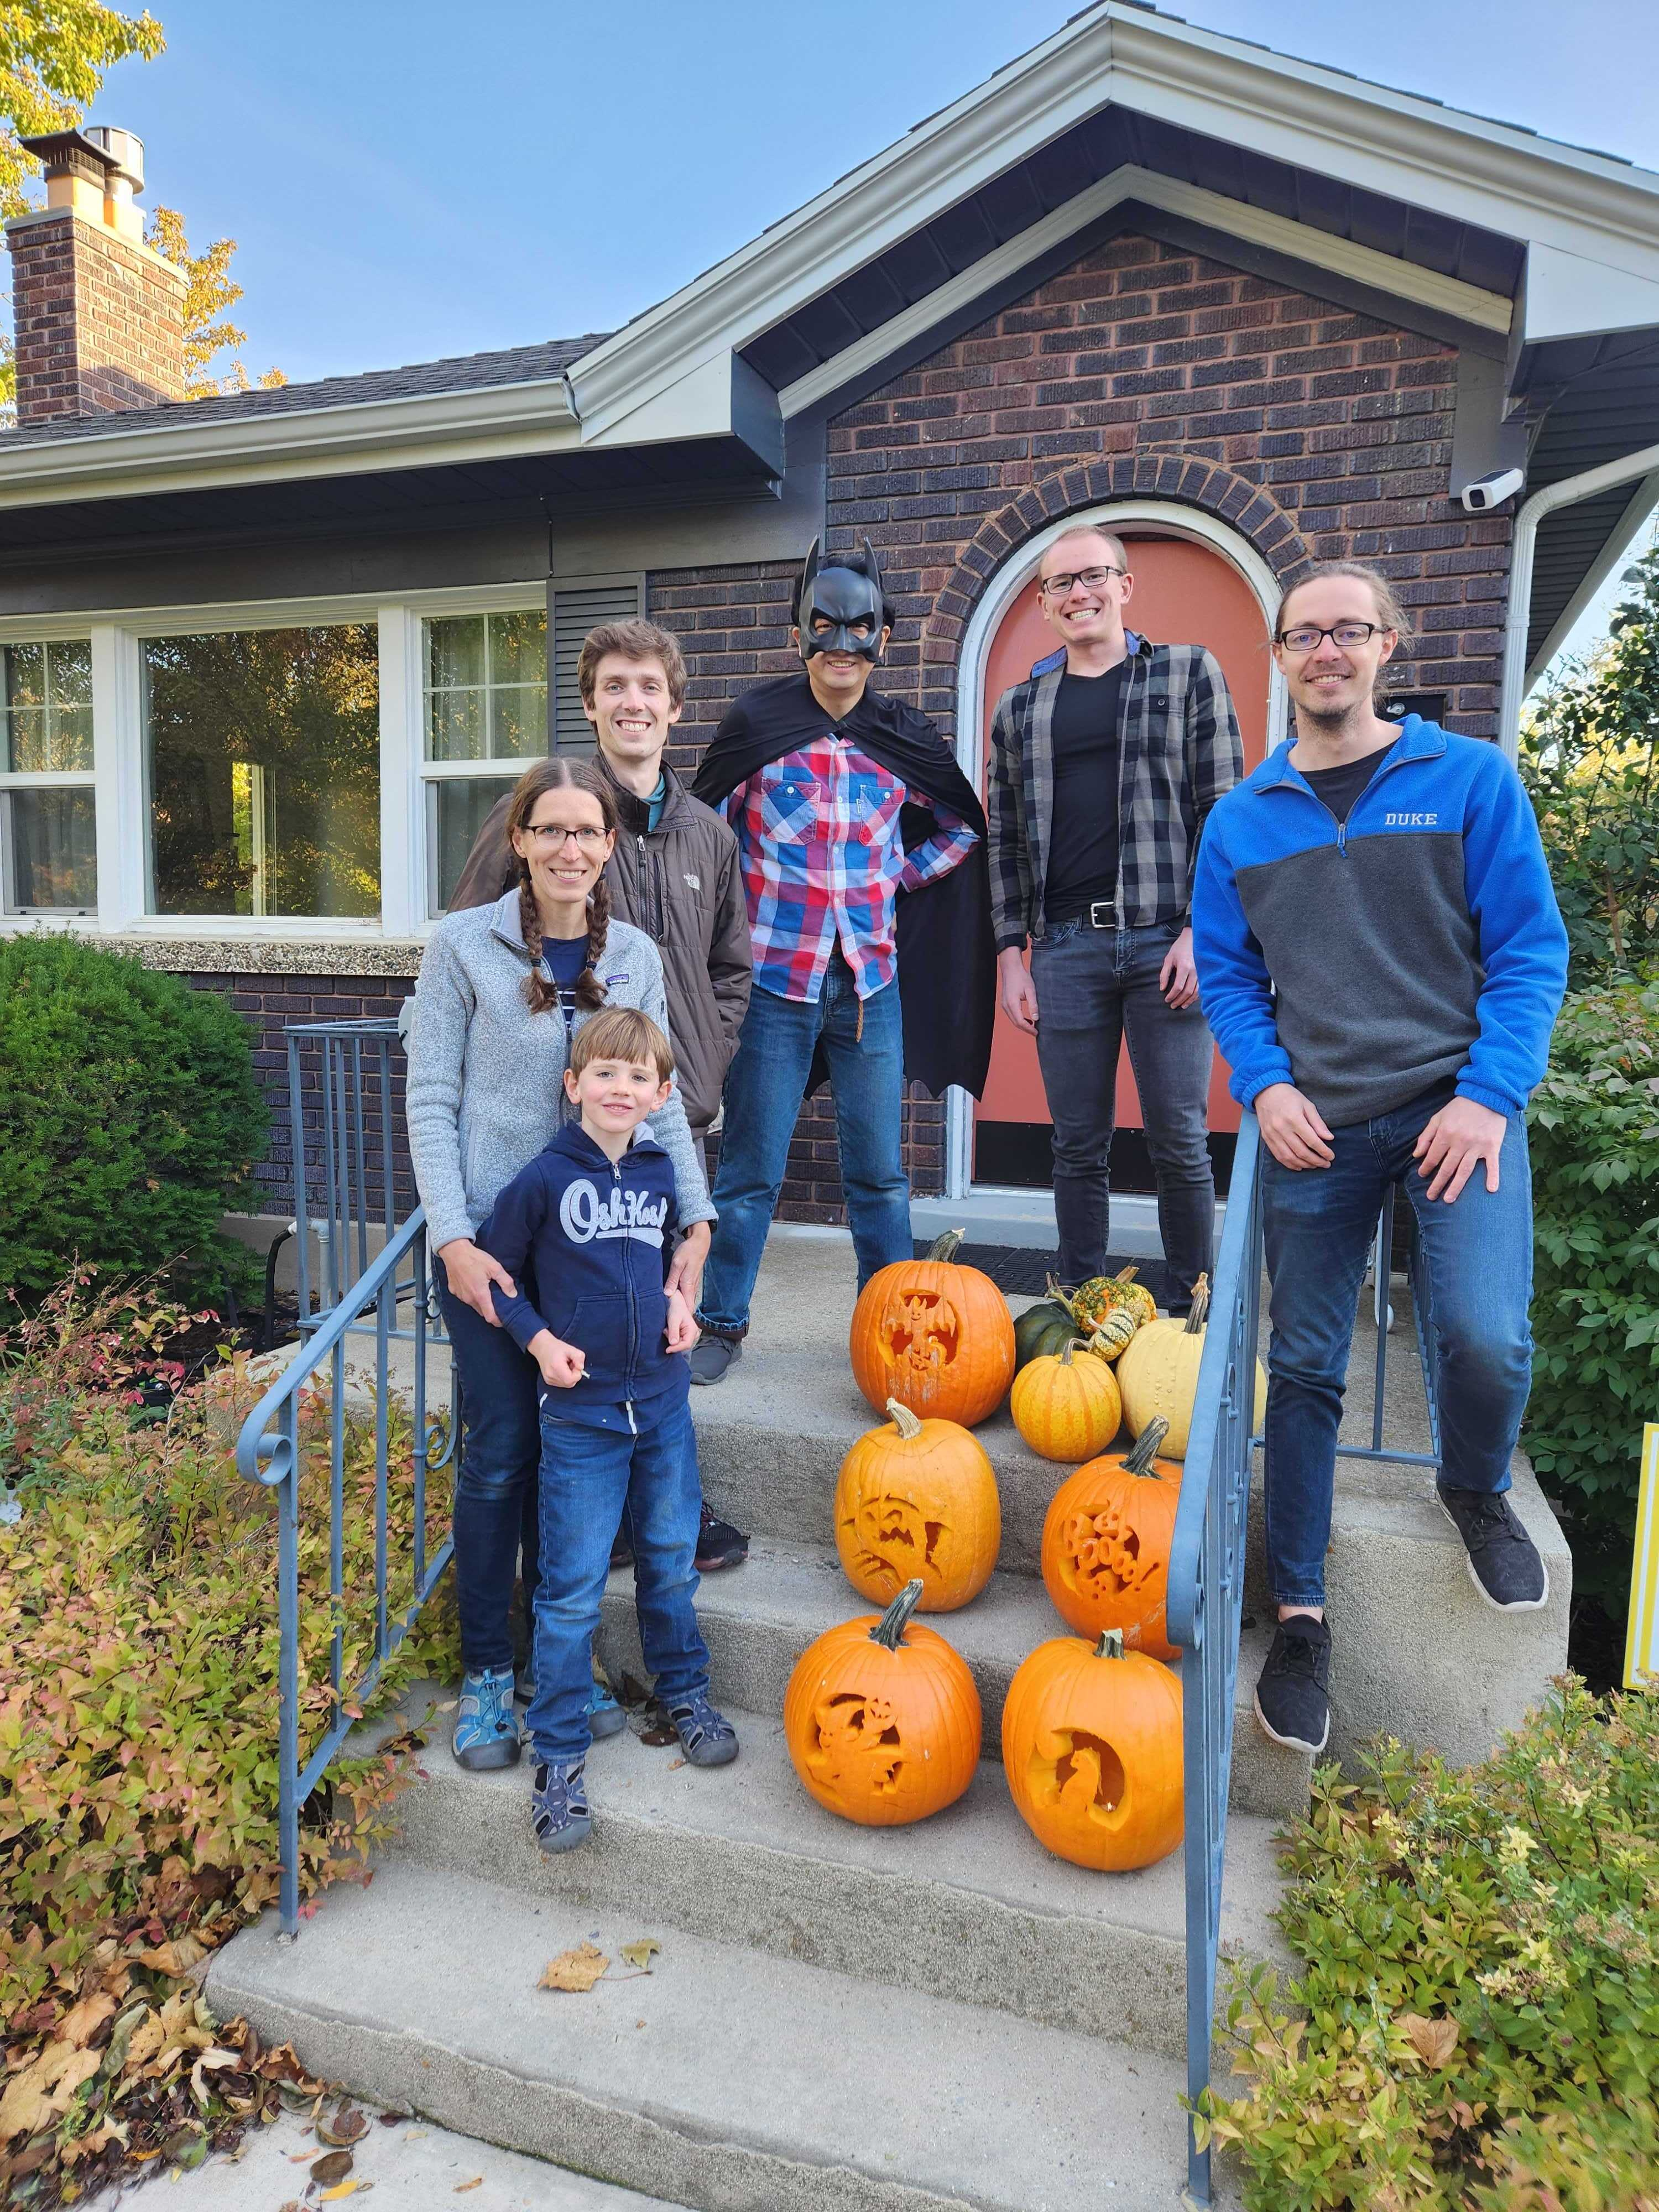
\includegraphics[scale=0.05]{figures/pumpkin.jpg}
        \hspace{0.25cm}
        
\includegraphics[scale=0.04]{figures/hiking.jpg}
    \end{center}

\end{frame}

\begin{frame}[t]
    \begin{figure}
        \begin{center}
            \begin{tikzpicture}
    \tikzstyle{node} = [circle, draw, thick, minimum size=0.7cm]
	\tikzstyle{edge} = [thick]
    \tikzstyle{gnode} = [rectangle, draw, thick, minimum width=1.6cm, minimum height=0.8cm, rounded corners=0.3cm]
    \tikzstyle{znode} = [circle, draw, minimum size=0.7cm, scale=0.83]

    \node (r) [node, fill=skyblue] {$r$};

    \node (u1) [node, fill=skyblue, above left=0.2cm and 0.2cm of r] {$c_1$};
    \node (u2) [node, fill=orange, above left=0.2cm and 0.2cm of u1] {$c_2$};

    \node (e1) [node, fill=vermillion, below left=0.2cm and 0.2cm of r] {$u_1$};
    \node (e2) [below left = 0.05cm and 0.05cm of e1] {$\dots$};
    \node (en) [node, fill=redpurple, below left=0.05cm and 0.05cm of e2] {$u_n$};

    \node (g11) [gnode, below right=0.2cm and 0.2cm of r] {$g_1$};
    \node (gi1) [gnode, right=0.2cm of g11] {$g_i$};
    \node (gn1) [gnode, right=0.2cm of gi1] {$g_m$};
    \node (f1) [node, fill=orange, right=0.3cm of gn1] {$f$};
    \node (fp1) [node, fill=bluegreen, right=0.3cm of f1] {$f'$};

    \node (g12) [gnode, above right=0.2cm and 0.2cm of r] {$g_1$};
    \node (gi2) [gnode, right=0.2cm of g12] {$g_i$};
    \node (gn2) [gnode, right=0.2cm of gi2] {$g_m$};
    \node (f2) [node, fill=orange, right=0.3cm of gn2] {$f$};
    \node (fp2) [node, fill=yellow, right=0.3cm of f2] {$f'$};

    \draw (r) edge [edge] (u1);
    \draw (u1) edge [edge] (u2);

    \draw (r) edge [edge] (e1);
    \draw (e1) edge [edge] (e2);
    \draw (e2) edge [edge] (en);


    \draw (r) edge [edge] (g11);
    \draw (g11) edge [edge] (gi1);
    \draw (gi1) edge [edge] (gn1);
    \draw (gn1) edge [edge] (f1);
    \draw (f1) edge [edge] (fp1);

    \draw (r) edge [edge] (g12);
    \draw (g12) edge [edge] (gi2);
    \draw (gi2) edge [edge] (gn2);
    \draw (gn2) edge [edge] (f2);
    \draw (f2) edge [edge] (fp2);

    \node (e1) [znode, fill=vermillion, below right=0.75cm and -0.56cm of g11] {$v_i^1$};
    \node (e2) [minimum size = 0.5cm, right=0.25cm of e1] {$\dots$};
    \node (en) [znode, fill=redpurple, right=0.25cm of e2] {$v_i^n$};
    \node (x) [znode, fill=bluegreen, right=0.25cm of en] {$x_i$};
    \node (y) [znode, fill=skyblue, right=0.25cm of x] {$y_i$};
    \node (z) [znode, fill=orange, right=0.25cm of y] {$z_i$};

    \draw (e1) edge [edge] (e2);
    \draw (e2) edge [edge] (en);
    \draw (en) edge [edge] (x);
    \draw (x) edge [edge] (y);
    \draw (y) edge [edge] (z);

    \draw ($(gi1.south west) + (0.1, 0.1)$) -- ($(e1.north) + (-0.27, 0.15)$);
    \draw ($(gi1.south east) + (-0.1, 0.1)$) -- ($(z.north) + (0.27, 0.20)$);
    \draw[thick, rounded corners=0.3cm] ($(e1.north west) + (-0.25, 0.25)$) rectangle ($(z.south east) + (0.25, -0.25)$);
\end{tikzpicture}

        \end{center}
    \end{figure}

\end{frame}

% \begin{frame}[t]
%     \frametitle{Thanks! :)}
%     Special Thanks to:

%     Dr. Sullivan

%     Brian Lavallee

%     Theory In Practice



% \end{frame}
